\section{Численные примеры}
\label{sec:validation}

\subsection{Граничная бернуллиевская модель}

Для расчёта ожидаемых длин используется ряд~\eqref{eq:dyadic-series}.
Математические ожидания для шумного учителя вычисляются полными
биномиальными суммами, а коэффициенты асимптотик --- одномерной
численной минимизацией.
Для ряда после $J$ порогов и $p=e^{-h}$ остаток ограничен величиной
\[
 3e^p\frac{e^{-p2^{J+1}}}{1-e^{-p2^{J+1}}}.
\]
Ряд обрывается при $p2^J\ge50$, что даёт остаток меньше $10^{-42}$;
суммы вычисляются в двойной точности. Минимумы локализуются на сетке и
уточняются ограниченной одномерной минимизацией.

\begin{table}[ht]
\centering
\caption{Численная оценка минимизатора замороженного протокола. Параметр $b$
не входит в ведущий коэффициент.}
\begin{tabular}{rrr}
\toprule
$a$ & $r_*$ & $A(a)$, бит/$\ln(1/\varepsilon)$\\
\midrule
0.10 & 5.780 & 1.252977\\
0.25 & 3.929 & 1.993603\\
0.50 & 2.922 & 2.976241\\
1.00 & 2.210 & 4.675413\\
\bottomrule
\end{tabular}

\label{tab:coef}
\end{table}

При $a=1/4$ получаем $r_*\approx3.928703$,
$h_*=a(r_*-1)\approx0.732176$ и $A(a)\approx1.993603$.
Ожидаемое число кандидатов в поздних пакетах приближается к
$e^{h_*}\approx2.079600$. Для $b=1$ ограничение $M=2$ немного повышает
ведущий коэффициент; при $M\ge2.079601$ этот численно найденный минимизатор
уже допустим. У совместного протокола ведущий коэффициент равен
$(1/4)/\ln2\approx0.360674$.

Для $N=63$, $a=1/4$, $b=1$ конечный риск всех сравниваемых расписаний равен
$\ln(1+0.25/64)\approx0.003899$ ната.

\begin{table}[ht]
\centering
\caption{Стоимость разных публичных расписаний при одинаковом конечном риске.}
\begin{tabular}{lrr}
\toprule
Размеры пакетов & Число сообщений & Ожидаемая длина, бит\\
\midrule
$3,12,48$ & 3 & 8.070631\\
$7,56$ & 2 & 9.303090\\
$63$ & 1 & 27.897764\\
63 пакета по одному & 63 & 66.297235\\
\bottomrule
\end{tabular}
\label{tab:N63}
\end{table}

Первое расписание --- оптимум рекурсии~\eqref{eq:dp}. Расписание $(7,56)$
минимизирует универсальную верхнюю оценку в этой задаче, но проигрывает
по фактическому математическому ожиданию. Таким образом, даже корректная
верхняя оценка может быть недостаточно точной для выбора протокола.

\begin{figure}[ht]
\centering
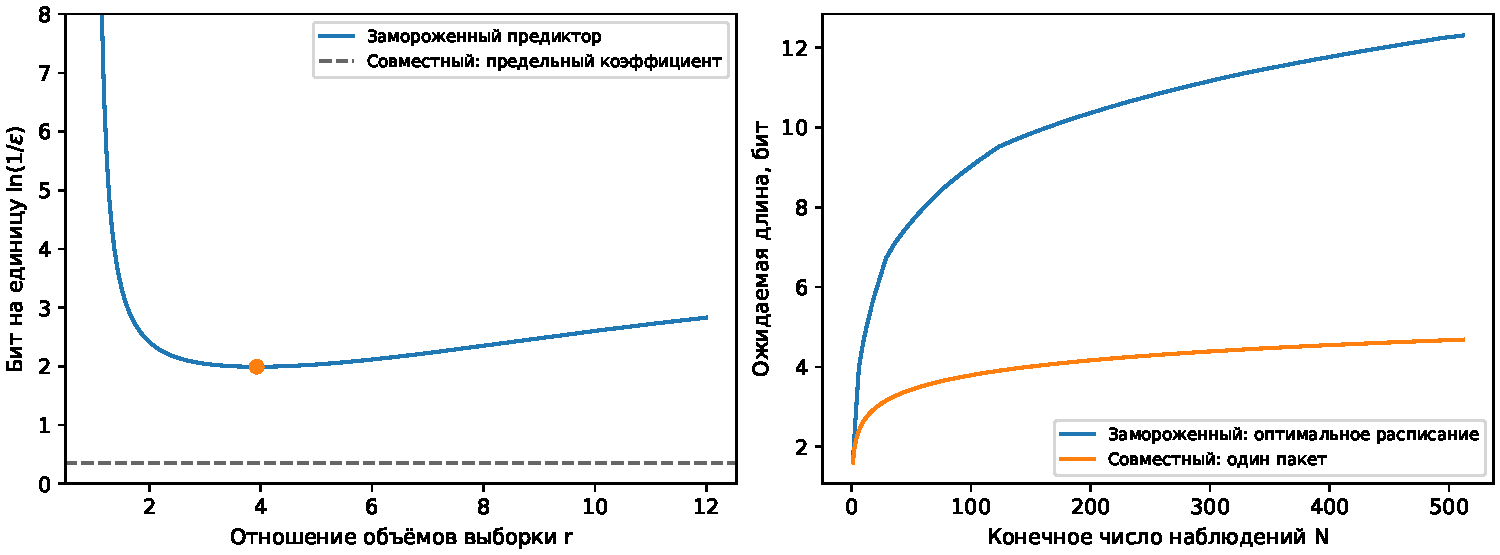
\includegraphics[width=\textwidth]{figures/protocol_costs.pdf}
\caption{Слева: ожидаемая стоимость замороженного пакета на единицу
логарифмического прироста объёма при $a=1/4$; пунктир --- ведущий коэффициент
совместного протокола. Справа: оптимальная конечная длина замороженного
протокола и стоимость одного совместного пакета при $b=1$.
Конечные длины совместного протокола могут быть заметно выше его ведущей
асимптотики из-за целочисленного кода индекса.}
\label{fig:protocol}
\end{figure}

Для оценки зависимости от второго параметра априорного распределения
на горизонте $N=256$
получены оптимальные длины $12.104019$, $10.839585$, $9.662267$ и $8.263138$
бита при $b=0.5,1,2,4$ соответственно. Это различие согласуется с тем, что
$b$ влияет на начальное состояние и ограниченный остаток, сохраняя $A(a)$,
как установлено в теореме~\ref{thm:optimal}.

\subsection{Шумный учитель}

При $q=0.20$, априорном распределении $\Beta(1,1)$ и $N=62$
ожидаемый конечный риск равен
приблизительно $0.007694$ ната. Точная
стоимость~\eqref{eq:conditional-index} и верхняя
оценка~\eqref{eq:universal-bound} выбирают разные расписания
(таблица~\ref{tab:noisy}). Оптимизация ожидаемой длины даёт экономию
$7.4715\%$. Результат относится к публичным детерминированным расписаниям
до $N=62$.

\begin{table}[ht]
\centering
\caption{Два критерия оптимизации. В обоих случаях конечный риск одинаков.}
\begin{tabular}{lrr}
\toprule
Размеры пакетов & Ожидаемая длина, бит & Сумма верхних оценок, бит\\
\midrule
$3,15,44$ & 10.255584 & 25.115133\\
$7,55$ & 11.083706 & 22.220445\\
\bottomrule
\end{tabular}
\label{tab:noisy}
\end{table}

\subsection{Проверка динамики и восстановления}

Для точного спуска при $\gamma=1,t_0=10$ и
$(a_0,b_0)=(0.2,0.05)$ расчёт до $T=2^{18}$ даёт
$D_T\approx0.149890564$. Оценка~\eqref{eq:imbalance-certificate}
ограничивает оставшееся уменьшение величиной $1.53\cdot10^{-10}$.
Соответствующий показатель $\alpha\approx0.299781128$ гарантированно меньше
единицы. Для старта $(1,0.05)$ получаем
$\alpha\approx1.896517056>1$. Таким образом, конечные значения дисбаланса
позволяют различить расходящуюся и сходящуюся суммы рисков.

В сбалансированном случае разность $s_T^{-1}-2\sum_{t<T}\eta_t$
стабилизируется в соответствии с доказательством теоремы~\ref{thm:factorized}.
При малых начальных нормах постоянный член в $s_T^{-1}$ остаётся существенным
на конечных горизонтах. Для аффинного ученика перебраны все $2^6$ суффиксов и оба
крайних начальных состояния; максимальная KL-ошибка составила
$0.0001528895$ ната, что ниже универсальной границы
$(9/7)4^{-6}\approx0.0003138951$.

Численная реализация проверена сравнением ряда для $L$ с прямой суммой
по геометрическому распределению, биномиального сведения PFR --- с перебором
бинарных строк длины три, а динамического программирования --- с перебором
всех $2^7$ расписаний до $N=8$.
